% ===================== PARTE 1: DISEÑO EXPERIMENTAL (diapositivas 6-23) =====================
\parte{Diseño experimental}{Diseño experimental: qué se midió\\y cómo se corrió}
  {Cuatro formas de correr las mismas pruebas, en dos máquinas, y por qué hizo falta cada una.}{s06}

\begin{frame}{Cuatro máquinas en juego: dos del paper y dos nuestras}
  \fuente{de Wolff et al., sección 6; equipo.txt del Ultra 9; 00\_entorno.txt del i5-10400}
  \footnotesize\renewcommand{\arraystretch}{1.15}
  \begin{tabularx}{\linewidth}{@{}>{\leavevmode\color{azul}\bfseries}p{0.13\linewidth}XXXX@{}}
    \toprule
    & \textbf{Paper, figura 5} & \textbf{Paper, figura 6} & \textbf{Réplica A} & \textbf{Réplica B}\\
    \midrule
    Procesador & 4 \por{} Xeon E7-8867 & Xeon w7-3465X & Core Ultra 9 285 & Core i5-10400\\
    Núcleos e hilos & 72 núcleos, 144 hilos & 28 núcleos, 56 hilos & 24 núcleos (8 P + 16 E), sin SMT & 6 núcleos, 12 hilos (SMT)\\
    Chips y memoria & 4 sockets, 4 nodos NUMA & 1 socket & 1 socket y 1 nodo NUMA; L3 de 36\,MB; RAM en 1 canal & 1 socket\\
    Sistema & --- & --- & Ubuntu 24.04, y Docker con Ubuntu 22.04 & WSL2 sobre Windows, Ubuntu 24.04\\
    Qué se midió & Rendimiento & Latencia & Todo: 4 tandas, controles, RAM, corrección & Corrección y una pasada rápida de \texttt{bench.cpp}\\
    \bottomrule
  \end{tabularx}
  \vfill
  \caja{Ninguna de nuestras máquinas tiene 4 sockets. Por eso se comparan \textbf{órdenes y proporciones} entre algoritmos, no Mop/s absolutos entre máquinas.}
  \nota{s07}
\end{frame}

\begin{frame}{Qué se corrió en cada máquina y de qué forma}
  \fuente{EXPLICACION.md, Partes 0, 4 y 6.6; resultados/david-ultra9-285/LEEME.md}
  \centering\scriptsize\renewcommand{\arraystretch}{1.12}
  \newcommand{\si}{\textcolor{verde}{\checkmark}}\newcommand{\nn}{\textcolor{gris}{---}}
  \begin{tabular}{@{}l*{6}{>{\centering\arraybackslash}p{0.105\linewidth}}@{}}
    \toprule
    & \multicolumn{5}{c}{\textbf{Core Ultra 9 285}} & \textbf{i5-10400}\\
    \cmidrule(lr){2-6}\cmidrule(l){7-7}
    & Docker, oficiales & Sin Docker, oficiales & Sin Docker, \texttt{bench.cpp} & \texttt{bench.cpp} alineado & Pasada rápida & Pasada rápida\\
    \midrule
    Rendimiento (figura 5) & \si & \si & \si & \si & \si & \si\\
    Latencia (figura 6) & \si{} 5 rondas & \si{} 15 rondas & \si & \nn & \si & \si\\
    Hilos fijados a núcleos & \si & \si & \si & \si & \nn & \nn\\
    Dos hilos en pares de núcleos & \si{} 3 rondas & \si{} 10 rondas & \si & \nn & \nn & \nn\\
    Memoria retenida & \si & \si & \nn & \nn & \nn & \nn\\
    Receta exacta, 10\,s \por{} 7 & \si{} 2 escen. & \si{} 6 escen. & \nn & \nn & \nn & \nn\\
    Tráfico real de RAM & \si & \nn & \si & \si & \nn & \nn\\
    ASan, TSan, boceto & \si{} rivales & \nn & \si{} rivales & \nn & \si & \si\\
    \midrule
    \textbf{Mediciones} & 3\,720 & 4\,660 & 2\,976 & 2\,160 & 168 & 168\\
    \bottomrule
  \end{tabular}
  \par\vfill\raggedright
  \caja{La pasada rápida es el mismo guion, \texttt{ejecutar\_pruebas.sh}, en las dos máquinas: es la comparación directa entre ellas.}
  \nota{s08}
\end{frame}

\begin{frame}{Más de 14\,000 mediciones, ninguna fallida}
  \fuente{EXPLICACION.md, Parte 0; datos de corrección de las dos máquinas}
  \centering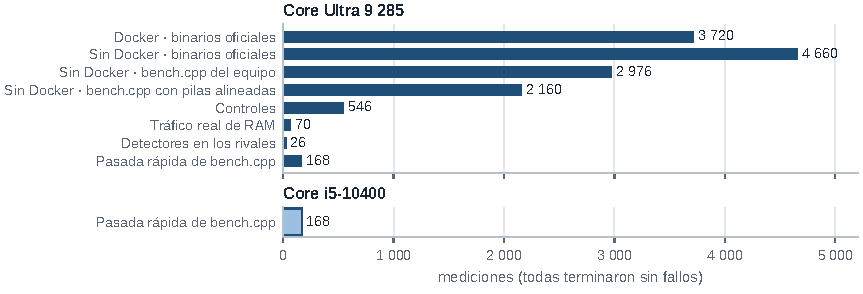
\includegraphics[width=\linewidth]{figuras/s09}
  \vfill\raggedright
  \caja{Todas las ejecuciones terminaron con código 0. Cada punto se midió en un proceso nuevo y en orden aleatorio.}
  \nota{s09}
\end{frame}

\begin{frame}{El flujo de trabajo, de principio a fin}
  \fuente{replica/completa: correr\_docker.sh, preparar.sh, correr\_nativo.sh, baterias.py, analizar.py; codigo/ejecutar\_pruebas.sh}
  \centering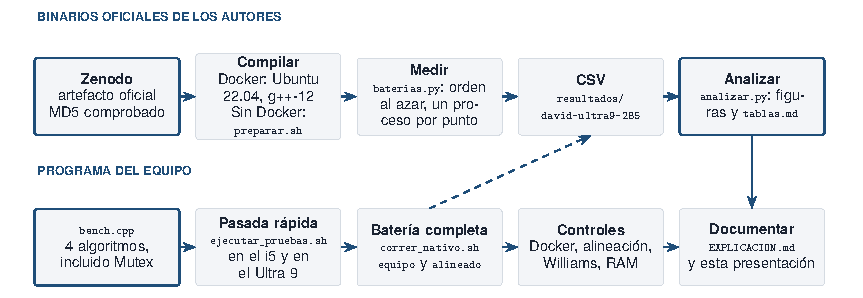
\includegraphics[width=\linewidth]{figuras/s10}
  \vfill\raggedright
  \caja{Todo se reanuda solo: si una medición se corta, se vuelve a lanzar la misma orden y salta lo ya medido.}
  \nota{s10}
\end{frame}

\begin{frame}{Paso 1 · El artefacto oficial, descargado de Zenodo}
  \fuente{EXPLICACION.md, Partes 4.2 y Referencias; replica/completa/correr\_docker.sh}
  \begin{columns}[T]
    \column{0.55\textwidth}
    \sub{Qué es}
    El paquete que publicaron los autores junto al paper: el código de los cinco algoritmos y los dos programas de medida.
    \par\medskip\footnotesize\renewcommand{\arraystretch}{1.15}
    \begin{tabularx}{\linewidth}{@{}>{\leavevmode\color{gris}}lX@{}}
      DOI & \texttt{10.5281/zenodo.11775182}\\
      MD5 & \texttt{\scriptsize e7e03425dfd426385a769788e5460fcd}\\
      Programas & \texttt{bench\_stack} (rendimiento) y el de latencia\\
      Rivales & Folly en el commit que fija el paper; Anderson en ParlayLib; Williams con \texttt{boost::atomic}\\
      Fijado por nosotros & Google Benchmark v1.8.3 y Google Test v1.14.0\\
    \end{tabularx}
    \column{0.41\textwidth}
    \caja{\textbf{Por qué así:} se mide el mismo código que midieron los autores. Una reimplementación propia podría ganar o perder por cómo está escrita, no por el algoritmo.}
    \par\medskip
    \aviso{El artefacto pide la rama \texttt{main} del día de Google Benchmark y Google Test, que ya no es la misma. Por eso se fijaron dos versiones concretas.}
  \end{columns}
  \nota{s11}
\end{frame}

\begin{frame}{Paso 2 · Compilar y medir dentro de Docker}
  \fuente{replica/completa/correr\_docker.sh y Dockerfile; EXPLICACION.md, Parte 9}
  \begin{columns}[T]
    \column{0.52\textwidth}
    \sub{Qué hace \texttt{correr\_docker.sh}}
    \begin{enumerate}\small
      \item Baja el artefacto y comprueba el MD5.
      \item Construye una imagen con Ubuntu 22.04 y g++-12, la misma base que usa el artefacto.
      \item Compila los binarios oficiales dentro.
      \item Lanza las baterías: unas 3 horas.
    \end{enumerate}
    \medskip
    \cmd{cd replica/completa\\bash correr\_docker.sh}
    \column{0.44\textwidth}
    \porque{Docker}{Docker \textbf{no es una máquina virtual}. El programa corre sobre el mismo núcleo de Linux y en la misma CPU; solo cambia lo que ve a su alrededor: bibliotecas, compilador y archivos. Sirve para tener el entorno de los autores sin tocar el sistema.}
    \par\medskip
    \aviso{Que Docker no altera los números había que demostrarlo. Se hizo en la parte 4.}
  \end{columns}
  \nota{s12}
\end{frame}

\begin{frame}{La receta oficial, sacada del artefacto}
  \fuente{EXPLICACION.md, Parte 4.2; artefacto de Zenodo}
  \begin{columns}[T]
    \column{0.6\textwidth}\footnotesize\renewcommand{\arraystretch}{1.18}
    \begin{tabularx}{\linewidth}{@{}>{\leavevmode\color{gris}}lX@{}}
      \toprule
      Orden & \texttt{bench\_stack -r 10 -s n -u u -i 7 -{}-peek=true -{}-threads=T -{}-alg=A}\\
      Algoritmos & \texttt{ivo} (Autores), \texttt{mine} (Anderson), \texttt{folly}, \texttt{jss-free} (Williams), \texttt{gnu} (Libstdc++)\\
      Asignador & \texttt{jemalloc}, cargado con \texttt{LD\_PRELOAD}\\
      Memoria & \texttt{numactl -i all}: repartida entre los nodos\\
      Hilos & 1, 18, 36, 54, 72, 108, 144, 180, 216\\
      Tamaño de pila & 20 elementos + $T/n$\\
      Resultado & Mediana de 7 ejecuciones de 10\,s\\
      \bottomrule
    \end{tabularx}
    \column{0.36\textwidth}
    \sub{Qué se mide}\small
    $n$ pilas concurrentes. En cada operación se elige una pila al azar: con probabilidad $u$\,\% se saca un elemento y se mete en otra; si no, se lee la cima.
    \par\medskip
    \caja{$n$ \textbf{pequeño} = mucha gente en poco sitio.\\ $u$ \textbf{grande} = mucha escritura.}
  \end{columns}
  \nota{s13}
\end{frame}

\begin{frame}{Adaptaciones a una máquina de 24 núcleos, y por qué}
  \fuente{EXPLICACION.md, Parte 4.3}
  \footnotesize\renewcommand{\arraystretch}{1.2}
  \begin{tabularx}{\linewidth}{@{}p{0.2\linewidth}p{0.27\linewidth}X@{}}
    \toprule
    \textbf{Paper} & \textbf{Réplica} & \textbf{Por qué}\\
    \midrule
    Hilos 1 a 216 & 1, 3, 6, 9, 12, 18, 24, 30, 36 & La lista del paper dividida entre 6: 24 es «toda la máquina», como 144; 36 es 1,5 veces, como 216\\
    7 \por{} 10\,s en un proceso & 5 rondas de 2\,s, un proceso nuevo por punto, en orden aleatorio & La figura 5 pasa de unas 5\,h a poco más de 1\,h, y el calor o una interrupción afectan a todos por igual\\
    $p = 56$ en latencia & $p = 1$, 24 y 56 & 24 son todos los núcleos reales; con 56 hay más hilos que núcleos\\
    Williams fuera de la latencia & Williams medido, compilado con \texttt{-mcx16} & El paper lo omite «porque su latencia casi siempre era mayor»: se comprobó en vez de creerlo\\
    \bottomrule
  \end{tabularx}
  \vfill
  \aviso{Recortar puede sesgar. Por eso se repitieron 30 puntos con la receta exacta de 10\,s \por{} 7: lo veremos en la parte 10.}
  \nota{s14}
\end{frame}

\begin{frame}{Fijar cada hilo a un núcleo sin tocar el binario}
  \fuente{replica/completa/herramientas/fijar\_hilos.c; EXPLICACION.md, Parte 5.4}
  \begin{columns}[T]
    \column{0.47\textwidth}
    \sub{Cómo funciona}\small
    \texttt{fijar\_hilos.c} es una librería pequeña que se carga delante del programa con \texttt{LD\_PRELOAD}. Intercepta la creación de cada hilo y lo ata al núcleo que le toca.
    \begin{itemize}
      \item El binario oficial \textbf{no se modifica}.
      \item Se comprobó leyendo el sistema: cada hilo estaba en su núcleo.
    \end{itemize}
    \medskip
    \caja{El experimento limpio: \textbf{los mismos 4 hilos}, del mismo tipo de núcleo, cada vez más lejos. Solo cambia la distancia.}
    \column{0.49\textwidth}\footnotesize\renewcommand{\arraystretch}{1.2}
    \begin{tabularx}{\linewidth}{@{}lX@{}}
      \toprule
      \textbf{Colocación} & \textbf{Qué imita}\\
      \midrule
      \texttt{E4-compacto} & 4 hilos en un clúster: todos en el mismo «socket»\\
      \texttt{E4-disperso} & uno en cada clúster: repartidos por los 4 «sockets»\\
      \texttt{P4} & 4 núcleos P: la máxima distancia\\
      \texttt{todos24} & toda la máquina, con los hilos fijados\\
      \texttt{sistema} & sin fijar: lo decide Linux, como en el paper\\
      \bottomrule
    \end{tabularx}
  \end{columns}
  \nota{s15}
\end{frame}

\begin{frame}{Antes de simular sockets, medir la distancia real entre núcleos}
  \fuente{matriz\_nucleos.csv (herramientas/latencia\_nucleos.cpp); EXPLICACION.md, Partes 5.2 y 5.3}
  \centering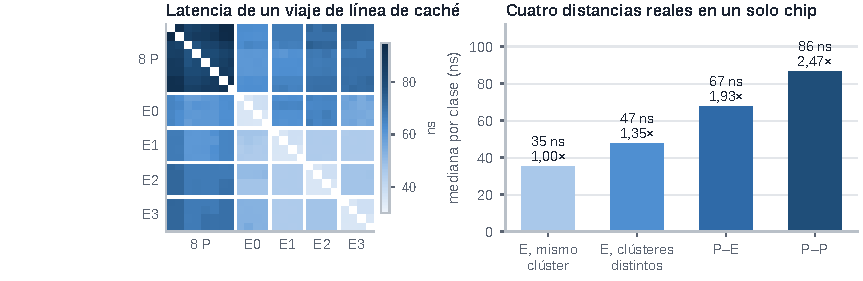
\includegraphics[width=0.92\linewidth]{figuras/s16}
  \vfill\raggedright
  \caja{Los 4 clústeres E se comportan como sockets en miniatura: cerca dentro y más lejos fuera. Pero el castigo es de \textbf{1,35\por}, frente a unas 3\por{} entre sockets Xeon (dato indirecto, de máquinas parecidas).}
  \nota{s16}
\end{frame}

\begin{frame}{Paso 3 · Sin Docker, primero con el programa del equipo}
  \fuente{EXPLICACION.md, Partes 6.6 y 8; replica/completa/correr\_nativo.sh}
  \begin{columns}[T]
    \column{0.52\textwidth}\small
    \sub{Por qué medir sin Docker}
    Para descartar que el contenedor cambiara los resultados. Si dentro y fuera dan lo mismo, Docker queda absuelto.
    \par\medskip
    \sub{Por qué se empezó por \texttt{bench.cpp}}
    Los binarios oficiales necesitan compilar Folly y ParlayLib fuera del contenedor. Al principio no compilaban: el sistema de permisos del asistente bloqueó \texttt{preparar.sh}, y lanzado a mano se paraba al configurar \texttt{bench\_stack}.
    \column{0.44\textwidth}
    \cmd{cd replica/completa\\SOLO\_DESCARGA=1 bash preparar.sh\\bash correr\_nativo.sh equipo}
    \begin{itemize}\footnotesize
      \item Autores, Libstdc++, Williams y Mutex; \textbf{Folly y Anderson no están}.
      \item Se le añadió \texttt{jemalloc} con \texttt{LD\_PRELOAD} y $n = \pot{6}$, sin tocar su código.
      \item 2\,976 mediciones, unas 1,5 horas.
    \end{itemize}
  \end{columns}
  \vfill
  \aviso{Aquí cambian dos cosas a la vez, el entorno y el programa. Separarlas exigió los controles de las partes 4 y 6.}
  \nota{s17}
\end{frame}

\begin{frame}{Paso 4 · Sin Docker con los binarios oficiales: la tanda nocturna}
  \fuente{EXPLICACION.md, Partes 8 y 9; replica/completa/pendientes.sh}
  \begin{columns}[T]
    \column{0.58\textwidth}\small
    \sub{El fallo, y su arreglo}
    El archivo de CMake de \texttt{fmt} sube 4 carpetas para hallar su raíz, pero el enlace de \texttt{preparar.sh} estaba a 3 carpetas de \texttt{install/fmt}: buscaba \texttt{install/lib/...} y no existía. Se arregló con dos enlaces.
    \par\medskip
    \sub{Qué hizo \texttt{pendientes.sh}}
    \begin{enumerate}\footnotesize
      \item Compilar los binarios oficiales fuera de Docker.
      \item Medir los 5 algoritmos: figura 5, afinidad y pares (10 rondas).
      \item Latencia con 15 rondas en vez de 5.
      \item Repetir \texttt{bench.cpp} con las pilas alineadas.
      \item Regenerar tablas y gráficas.
    \end{enumerate}
    \column{0.38\textwidth}
    \vspace{4mm}
    \cifra{4\,h 44\,min}{noche del 6 al 7 de noviembre de 2026,\\de 23:07 a 03:51}\par\bigskip\bigskip
    \cifra{0}{fallos; \texttt{comprobar\_final.py} confirmó\\que no faltaba ninguna fila}
  \end{columns}
  \nota{s18}
\end{frame}

\begin{frame}{Dentro y fuera de Docker cambia más que Docker}
  \fuente{EXPLICACION.md, Parte 6.6}
  \begin{columns}[T]
    \column{0.42\textwidth}\small\renewcommand{\arraystretch}{1.15}
    \begin{tabular}{@{}lll@{}}
      \toprule
      & \textbf{Con Docker} & \textbf{Sin Docker}\\
      \midrule
      g++-12 & 12.3.0 & 12.4.0\\
      glibc & 2.35 & 2.39\\
      Boost & 1.74 & 1.83\\
      jemalloc & 5.2.1 & 5.3.0\\
      Folly & \texttt{getdeps.py} & CMake directo\\
      \bottomrule
    \end{tabular}
    \column{0.54\textwidth}
    \caja{Si un resultado cambia al salir de Docker, no se puede culpar a Docker sin más: cambian \textbf{cinco piezas} a la vez.}
    \par\medskip
    \caja{Y si nada cambia, es que esas cinco piezas juntas tampoco importan aquí.}
  \end{columns}
  \vfill
  \porque{por qué importa Boost}{El Williams del artefacto usa \texttt{boost::atomic}. Un cambio de versión de Boost es el primer sospechoso de la única diferencia grande entre las dos tandas, Williams entre clústeres (parte 9). Es una sospecha: no se midió.}
  \nota{s19}
\end{frame}

\begin{frame}{El programa del equipo no es el programa oficial}
  \fuente{EXPLICACION.md, Parte 6.6}
  \footnotesize\renewcommand{\arraystretch}{1.15}
  \begin{tabularx}{\linewidth}{@{}>{\leavevmode\color{gris}}p{0.2\linewidth}XX@{}}
    \toprule
    & \textbf{\texttt{bench\_stack}, oficial} & \textbf{\texttt{codigo/bench.cpp}, del equipo}\\
    \midrule
    Algoritmos & Los 5 del paper & Autores, Libstdc++, Williams y Mutex\\
    \rowcolor{ambarsuave}\color{tinta}\bfseries Pilas en memoria & \textbf{Cada una en su sitio: \texttt{alignas(128)}} & \textbf{Seguidas, sin alinear}\\
    Nodos por pila & 20 + $T/n$ & 16, o 2 si $n > 10$\\
    Generador de azar & Uno rápido & \texttt{mt19937\_64}, más lento\\
    Compilación & \texttt{-O3} & \texttt{-O2}\\
    Williams & Con \texttt{boost::atomic} & Con \texttt{std::atomic}\\
    Autores & Versión del artefacto: la cuenta sube & Versión publicada: la cuenta baja\\
    \bottomrule
  \end{tabularx}
  \vfill
  \caja{Son dos programas escritos por personas distintas. Cuando coinciden, el resultado es sólido. Cuando no, la diferencia está en el programa, y hay que encontrarla.}
  \nota{s20}
\end{frame}

\begin{frame}{El i5-10400: cómo se corrieron sus pruebas}
  \fuente{codigo/ejecutar\_pruebas.sh y correr\_tsan.sh; 00\_entorno.txt del i5-10400}
  \begin{columns}[T]
    \column{0.55\textwidth}
    \sub{Entorno}\footnotesize
    \begin{tabular}{@{}>{\leavevmode\color{gris}}ll@{}}
      Sistema & WSL2 sobre Windows (Linux 6.18), Ubuntu 24.04\\
      Compilador & g++ 13.3\\
      Hilos & 12 (6 núcleos con SMT)\\
    \end{tabular}
    \par\medskip\normalsize
    \sub{Qué hace \texttt{ejecutar\_pruebas.sh}}
    \begin{enumerate}\footnotesize
      \item Demo del código de los autores.
      \item ASan con 8, 12 y 16 hilos; TSan con \texttt{setarch -R}.
      \item El boceto y dos variantes rotas.
      \item \texttt{bench.cpp}: rendimiento, 1\,s por punto, hilos 1 a 18.
      \item \texttt{bench.cpp}: latencia, 100\,000 muestras, $p = 1$ y 12.
    \end{enumerate}
    \column{0.41\textwidth}
    \cmd{cd codigo\\bash ejecutar\_pruebas.sh \textbackslash\\\ \ ../replica/resultados/<nombre>-<cpu>}
    \par\medskip
    \caja{El \textbf{mismo guion} se corrió en el Ultra 9 (\texttt{correccion/}): mismos parámetros y misma versión del compilador.}
    \par\medskip
    \aviso{Una sola pasada de 1\,s por punto: solo valen las diferencias grandes.}
  \end{columns}
  \nota{s21}
\end{frame}

\begin{frame}{Controles: un experimento pequeño para cada duda}
  \fuente{replica/completa: controles.sh, control\_williams.sh, herramientas/; EXPLICACION.md, Partes 6.1 a 6.7}
  \footnotesize\renewcommand{\arraystretch}{1.13}
  \begin{tabularx}{\linewidth}{@{}p{0.3\linewidth}Xl@{}}
    \toprule
    \textbf{Control} & \textbf{Qué aísla} & \textbf{Dónde se ve}\\
    \midrule
    Mismo código dentro y fuera de Docker & Docker por sí solo: 48 puntos alternados, 3 rondas & \hyperlink{parte4}{Parte 4}\\
    \texttt{alignas(128)} en una copia de \texttt{bench.cpp} & La colocación de las pilas en memoria & \hyperlink{parte6}{Parte 6}\\
    Williams con \texttt{std::atomic} y con \texttt{boost::atomic} & La biblioteca atómica de Williams & \hyperlink{parte9}{Parte 9}\\
    Contadores de la controladora de memoria & El tráfico real de RAM: \texttt{medir\_memoria.py}, \texttt{alinear\_memoria.py} & Partes 3 y 6\\
    Detectores en los rivales & Que ningún rival gane usando memoria liberada & \hyperlink{parte2}{Parte 2}\\
    Contador en una copia del código de los autores & Los intentos reales de la recarga & \hyperlink{parte2}{Parte 2}\\
    Receta exacta, 10\,s \por{} 7 & El efecto de recortar la duración & \hyperlink{parte10}{Parte 10}\\
    Valores del paper sacados del PDF vectorial & Comparar número contra número (\texttt{extraer\_fig5.py}) & Partes 3 y 7\\
    \bottomrule
  \end{tabularx}
  \nota{s22}
\end{frame}

\begin{frame}{Calidad de las mediciones y tres reglas para leerlas}
  \fuente{EXPLICACION.md, Partes 6 y 8}
  \begin{columns}[T]
    \column{0.47\textwidth}
    \sub{Calidad}
    \begin{itemize}\footnotesize
      \item 0 ejecuciones fallidas en todas las tandas.
      \item Con Docker: temperatura mediana de 75\,°C; solo 5 de 3\,720 llegaron a 90\,°C o más.
      \item Sin Docker: 26 de 9\,796 a 90\,°C o más; máximo, 99\,°C. Repartidas, no se descartaron.
      \item Dispersión típica entre rondas: 1\,\%; en los puntos más ruidosos, 8\,\%.
      \item PC de escritorio sin aislar y con la frecuencia sin fijar: el orden aleatorio reparte las interferencias.
    \end{itemize}
    \column{0.49\textwidth}
    \sub{Tres reglas de lectura}
    \begin{enumerate}\footnotesize
      \item \textbf{Se comparan algoritmos, no máquinas.} La CPU es casi diez años más moderna que los Xeon del paper.
      \item \textbf{«0,50\por» es «rinde la mitad que Autores».} Así se compara sin que importe la máquina.
      \item \textbf{Una diferencia pequeña es un empate.} Recortar la duración movió algunos puntos hasta un 21\,\%: solo cuentan las diferencias de 2 o 3 veces.
    \end{enumerate}
  \end{columns}
  \nota{s23}
\end{frame}
